\section{Create an OpenFoam cluster on AWS}

Large calculations require a lot of RAM memory and processor's cores. Without required memory the calculations cannot be carried out. With a small number of processors it woulde take a lot time. Sometimes, a signle instance is insufficient to make for example CFD calculations. It is possible to merge a few istances to make a larger one.

Create the OpenFoam cluster will be presented. The bash script has been created to automate calculations.

\subsection{Ssh Agent}

A premission master instance to slave instances is given by publikey (.pem) through ssh agent. To enable connect to instances without -i parameter, this script should be run:

\begin{figure}[h!]
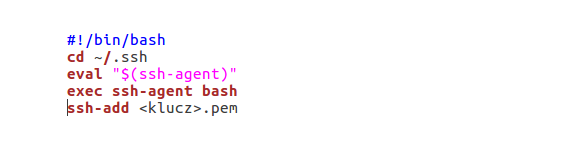
\includegraphics[width=\textwidth]{img/ssh_agent}
\caption{SSH Agent script}
%\label{fig:boat1}
\end{figure}

Lines begin with "eval" and "exec" are necesserly when something is going wrong.

\subsection{Sharing the Master Instance Volume}

Next script share the master instance volume to slave instances. All data is storage in master instance, slave instances share memory and processors' cores, but all data are save in master instance.

\begin{figure}[h!]
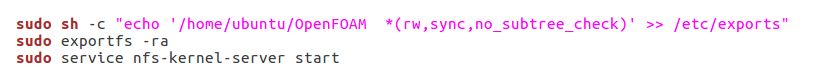
\includegraphics[width=\textwidth]{img/share_volume}
\caption{Share volume script}
%\label{fig:boat1}
\end{figure}

\subsection{Mounting the Master Volume from Slaves}

Next